\subsubsection{Representacion de la Matriz de Transicion (RODRI/FEDE)}
Este experimento lo pueden hacer directo o usando al PageRank. Si pueden, implementen todas las representaciones de matrices y luego comparen el tiempo de computo del producto N veces. Comparen la matriz normal vs el resto. Discutan que en páginas web la cantidad de vertices del grafo se va al carajo, pero para deportes es super acotada, asi que la eleccion de estructura no afecta tanto.

Aca podes argumentar que lo que domina al metodo de la potencia es la cantidad de productos, asi que no hace falta probar PageRank directo. Igual si queres metelo con pagerank de una, a fin de cuentas es lo mismo.

\begin{figure}[h]
\centering
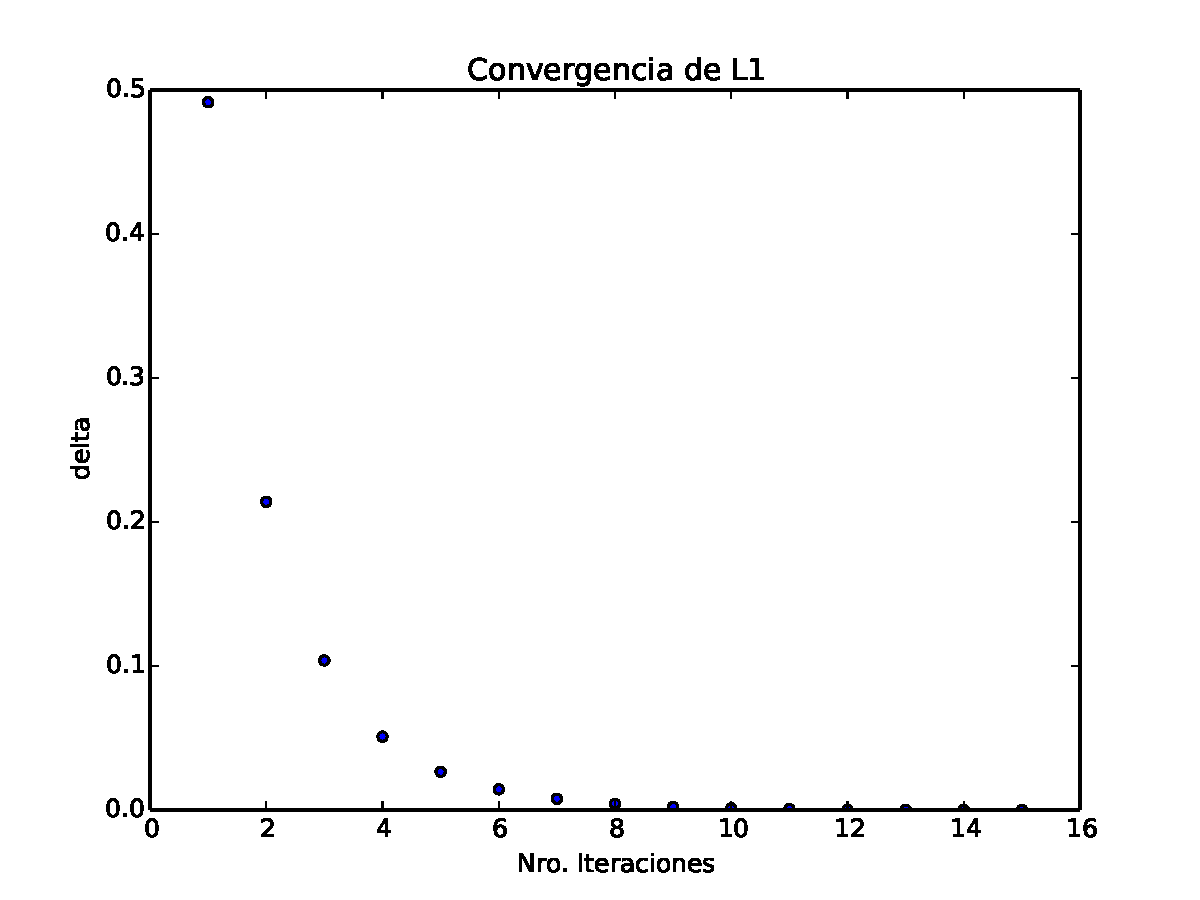
\includegraphics[scale=0.7]{images/conv_2265.pdf}
\caption{Tiempos de ejecución según cantidad de webs.}
\label{timePageRank}
\end{figure}

\begin{figure}[h]
\centering
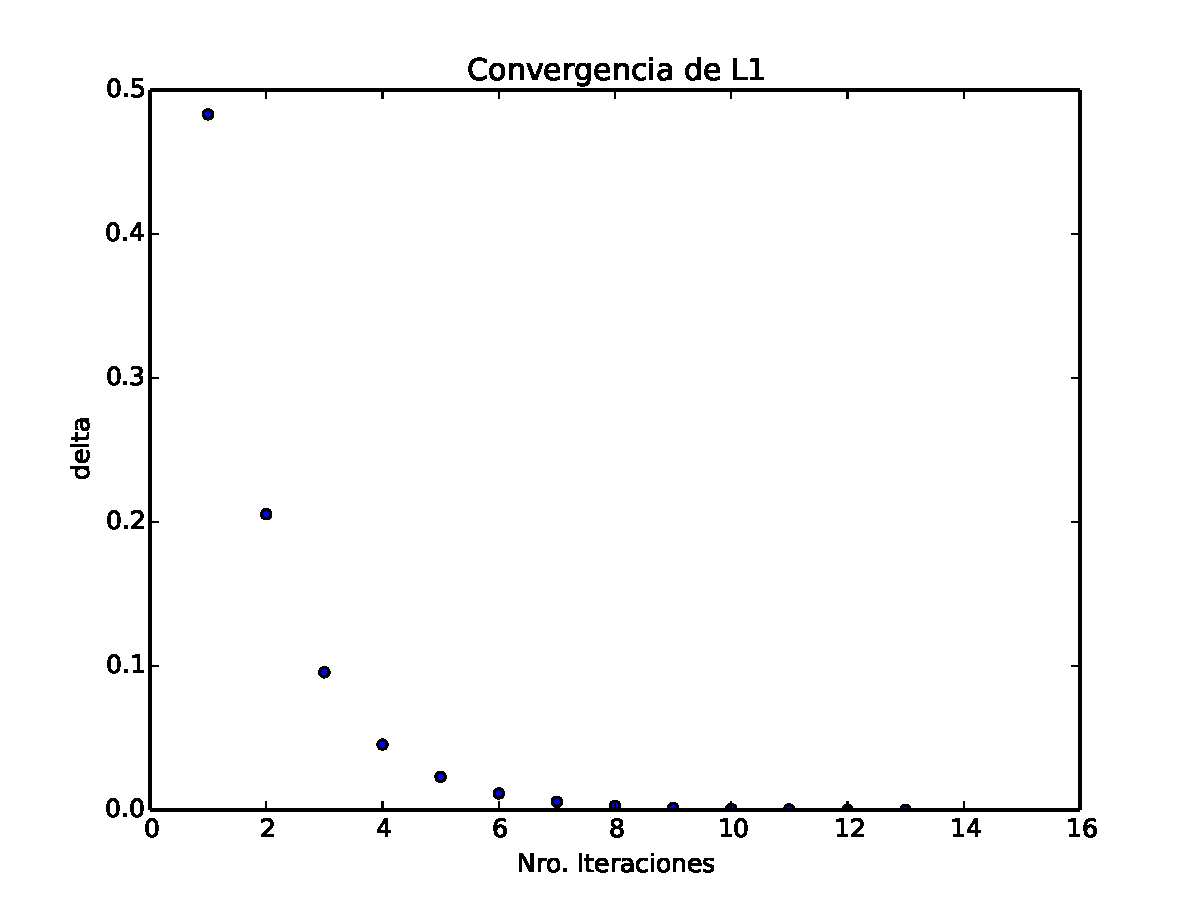
\includegraphics[scale=0.7]{images/conv_5000.pdf}
\caption{Tiempos de ejecución según cantidad de webs.}
\label{timePageRank}
\end{figure}
